\section{Maverick Flow Phase}
\label{sec:flow}

\begin{figure}[tb]
	\centering
	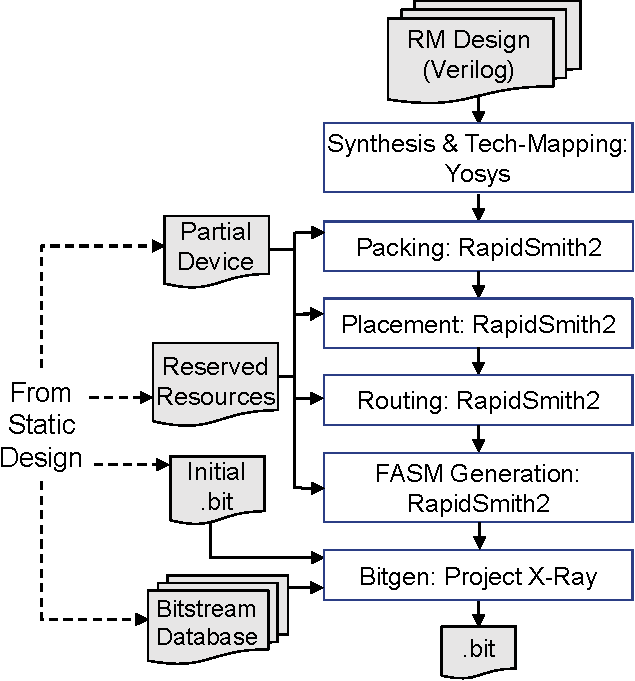
\includegraphics[height=.8\columnwidth]{figures/maverick_flow.pdf}
	\caption{Maverick Flow Phase}
	\label{fig:maverick_flow}
\end{figure}

The second phase is the stand-alone Maverick flow, which compiles RM designs to the PR region, independently of any vendor tools.
The Maverick flow is shown in \figurename~\ref{fig:maverick_flow} and consists of six major steps: synthesis, packing, placement, routing, FASM (FPGA Assembly) file generation, and bitstream generation.
This section describes each of these steps in turn.

\subsection{Synthesis and Tech-Mapping: Yosys}

\begin{figure}[tb]
	\centering
	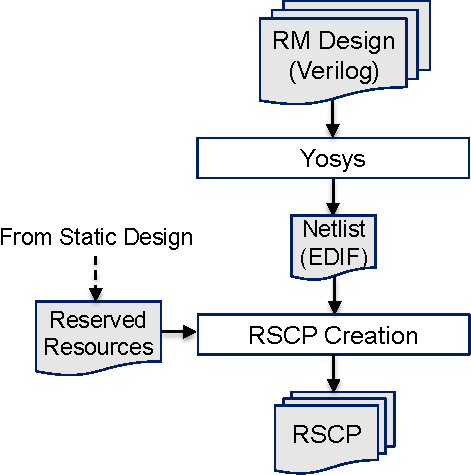
\includegraphics[width=0.58\columnwidth]{figures/synthesis}
	\caption{The Synthesis and Tech-Mapping Step in Maverick}
	\label{fig:synthesis}
\end{figure}

The first step of the Maverick flow is synthesis and tech-mapping. 
Maverick performs this using Yosys \cite{Wolf:2013}, a powerful open source framework for register-transfer level (RTL) synthesis that is capable of tech-mapping to Xilinx 7-Series devices. 
\figurename~\ref{fig:synthesis} shows how Yosys is used in the Maverick flow. 

Maverick executes Yosys using a synthesis script that combines several standard Yosys subsystems to optimize and tech-map the RM Verilog design to the Xilinx 7-Series architecture. 
At the time of this work, both Yosys and Project X-Ray support only a subset of 7-Series device features.
Because of this, the synthesis script limits Yosys to mapping designs to slice structures (containing lookup tables [LUTs] and flip-flops) only.
%As support for additional device features is added to these two tools, the entire Maverick flow will be able to support a larger subset of the device.  

Yosys produces a tech-mapped design in the form of a flattened EDIF netlist.
This netlist is made up of logical Xilinx 7-Series cells (e.g., LUTs and flip-flops) that are all interconnected by logical nets.   
The Maverick flow packages the EDIF netlist and the reserved resource list (from the static design) into a RapidSmith Checkpoint (RSCP), which is suitable for processing by RapidSmith2.

\subsection{RapidSmith2 Design Import}
\begin{figure}
	\centering
	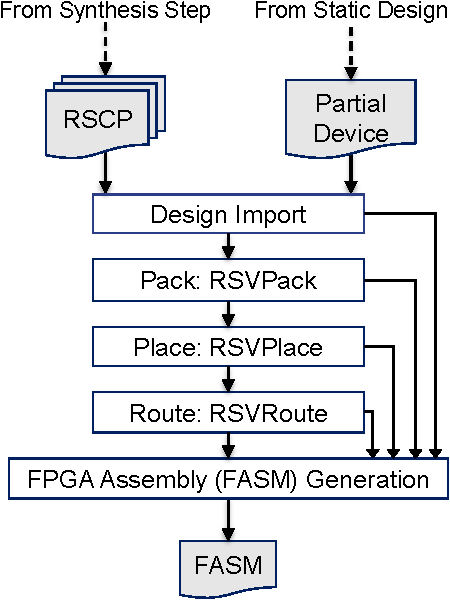
\includegraphics[width=0.58\columnwidth]{figures/rs2_steps.pdf}
	\caption{The RapidSmith2-based Steps in Maverick}
	\label{fig:rs2_steps}
\end{figure}

As shown in \figurename~\ref{fig:rs2_steps}, a set of RapidSmith2-based programs are next used to physically implement the tech-mapped design.
The next step in the Maverick flow is thus to import the tech-mapped design from Yosys into RapidSmith2.

To do so, the partial device model (from the static design) is first imported, providing RapidSmith2 with necessary details about the resources available in the PR region. 
The RSCP generated from the previous synthesis and tech-mapping step is also imported.
The EDIF netlist contained in the RSCP is translated for use within RapidSmith2 and the reserved resource list is then parsed to create internal data structures that mark the resources reserved by the static design.

\subsection{Packing: RSVPack}
The Maverick flow next packs the design, grouping related cells from the netlist into relatively placed clusters.
The created clusters correspond to sites in the Xilinx architecture, most of which are slices.
These sites are composed of internal site wires and Basic Elements of Logic (BELs).
These BELs include logic BELs, such as LUTs and flip-flops, and also routing BELs, which are programmable routing muxes.

The Maverick flow packs designs using the RSVPack algorithm \cite{Haroldsen:2016}.
RSVPack specifically targets Xilinx architectures, allowing it to produce results that take advantage of unique architectural features.
The version of RSVPack used in this work has been modified to work within PR regions---specifically to recognize partition pins.

The RSVPack algorithm repeatedly packs the site clusters with cells. 
To ensure that the clusters are valid for the target architecture, a series of tests is run each time a cell is added to a cluster.
Each time a cell is added to a cluster, a series of tests is run to verify that the cluster is valid for the architecture.
After all the cells in the design have been packed, RSVPack performs the intra-site routing of the nets; i.e., it routes all the portions of the nets that are inside the site clusters.
It does this by configuring the site clusters' internal routing BELs.

\subsection{Placement: RSVPlace}
Once packing completes, the Maverick flow places the design using a modified version of RSVPlace \cite{Haroldsen:2016}, also built on top of RapidSmith2. 
%RSVPlace is a non-timing driven placer. 
It first performs a quick random placement of the clusters created in the packing step.
This is followed by the execution of a simulated annealing placer using a wire-length based cost function.
The cost function and annealing schedule used by this placer are both based on VPR's placer \cite{Betz:1997}.
Furthermore, the placer uses the partial device model (created in the static design phase), preventing the placer from using any resources outside the PR region.

As mentioned previously and shown in \figurename~\ref{fig:partPins}, some resources within the PR region may be used by the static region and are marked as reserved.
RSVPlace was modified to not utilize any of these resources.
This is necessary for a PR-aware placer because in some initial static designs produced by Vivado the static logic may use a site within a PR region as a ``route-through''.
When a site is used as a route-through, the entire site is used to route a net from one of the site's input pins to one of its output pins.
Sites used by the static design as route-throughs are thus unavailable for use by the placer.

Once RSVPlace completes, all logical cells of the design have been assigned to specific locations in the PR region.
These assignments are saved internally within RapidSmith2, giving a global router the information it needs to complete the routing of the design.

\subsection{Routing: RSVRoute}
The Maverick flow then uses a new router called RSVRoute, also built upon the RapidSmith2 framework, to route the nets of the design. 
RSVRoute is primarily based on Pathfinder \cite{Ebeling:1995} and is the first full router created using RapidSmith2.
To construct routes, it turns on programmable interconnect points (PIPs) contained within the FPGA interconnect.

RSVRoute iteratively routes the unrouted and congested nets in the design until all nets are routed and uncongested.
Like VPR \cite{Betz:1997}, the cost for a net to use a congested routing resource is the product of the base cost, present congestion penalty, and historical congestion penalty of that routing resource.
Also like VPR, the present congestion penalty of a routing resource is updated every time a net is routed and the historical congestion penalty is updated between routing
iterations.
During every routing iteration, RSVRoute uses the A* shortest path algorithm \cite{Hart:1968} to quickly identify a shortest path, based on wire-length, for each congested net.

RSVRoute has two unique characteristics to support PR.
First, it must create routes while avoiding PIPs that are reserved by the static design. 
Second, in an RM design, nets connect to not only logic block pins but also to partition pins, which are physically implemented as wire segments within the PR region.
RSVRoute interconnects logic block pins with these partition pins; this feature is essential for completing the routing of RM designs contained within PR regions.

\subsection{FASM Generation: RapidSmith2}
\label{sec:fasm}

The next step in the Maverick flow is to generate an FPGA Assembly (FASM) file \cite{PrjXray}.
This is a human-readable text file that contains a list of low-level instructions to configure the FPGA's resources.
Specifically, FASM files contain instructions to perform functions such as enabling PIPs in interconnect tiles, configuring LUTs, and configuring other BEL and site-level properties.
The FASM format contains enough information so that in conjunction with the bitstream database and initial partial bitstream, a new valid partial bitstream can be generated for an RM design.

As shown in \figurename~\ref{fig:rs2_steps}, data structures created by each of the preceding RapidSmith2-based programs are used to generate the FASM file.
Many of the FASM instructions are straightforward to generate due to the detailed partial device model imported into RapidSmith2.
For instance, to determine the interconnect PIPs to turn on, the FASM generator iterates through route tree data structures (created by RSVRoute).
Each time an enabled PIP is encountered, the FASM generator writes a corresponding instruction to the output FASM file.
An example of such an instruction is shown below: 
\begin{center}
	\texttt{INT\_L\_X38Y16.SE2BEG1 LOGIC\_OUTS\_L1}
\end{center}
\noindent In this example, the starting point for the connection to be turned on is the wire ``LOGIC\_OUTS\_L1'', located in the interconnect tile ``INT\_L\_X38Y16'', and the PIP to be turned on is the one which connects that wire to the wire ``SEG2BEG1''. 
It is similarly straightforward to configure routing BELs.

Writing the instructions to configure sites and their logic BELs is more challenging, mainly because EDIF netlists represent only the logical properties associated with the cells in the netlist and not the physical site-wide and BEL properties.
This necessitates the translation of logical properties associated with cells to physical properties associated with sites and BELs.
One example of a property that requires such translation is whether all the flip-flops in a slice use a synchronous or an asynchronous reset.
Another example has to do with LUT programming. 
Routing may reorder a LUT's input pin connections to help with routing congestion; this requires the LUT equation be reformulated.
Additional handling is also necessary for fracturable 6-input LUTs and LUT RAM initialization.
All of this handling must be done in order to produce correct FASM instructions.

An important final step for the FASM generator is to process the resources that were reserved by the static design, as shown in \figurename~\ref{fig:partPins}.
This includes turning on any PIPs used to connect the static design to the PR design at partition pins as well as any other PIPs that may have been reserved by the static design.
 
\subsection{Bitstream Generation: Project X-Ray}
\begin{figure}
	\centering
	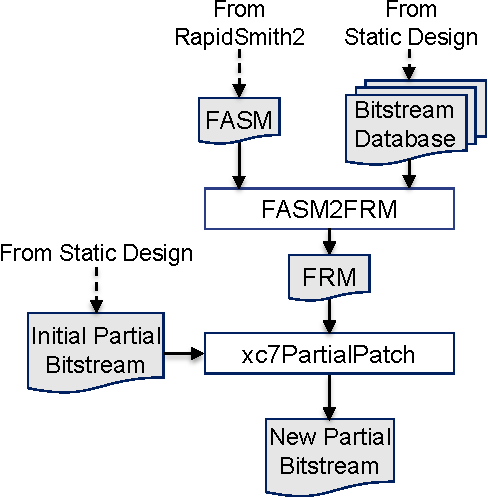
\includegraphics[width=0.62\columnwidth]{figures/bitgen.pdf}
	\caption{The Partial Bitstream Generation Step in Maverick}
	\label{fig:bitgen}
\end{figure}

Finally, the Maverick flow generates the partial bitstream for the RM design.
To do so, it uses the generated FASM file as well as the Project X-Ray bitstream database and initial partial bitstream (both from the static design). 
\figurename~\ref{fig:bitgen} shows how Project X-Ray is used to perform this step.

First, Project X-Ray's FASM2FRM Python script uses the bitstream database to convert the FASM file to a FRM file, which contains the configuration data for every individual bitstream frame within the PR region.
Then, to generate the partial bitstream, the FRM file and the initial partial bitstream are used as inputs to the xc7PartialPatch C++ program, created as a part of this work\footnote{This program is based on the original Project X-Ray xc7Patch program, but with significant modifications to support partial bitstreams.}.
The xc7PartialPatch program patches the initial partial bitstream with the contents of the FRM file, producing a new partial bitstream for the fully implemented RM described by the FRM file.
This resulting partial bitstream can then be configured onto the FPGA once it has first been programmed with the full-device static bitstream.
